\subsection{Run-length coding}
\paragraph*{Basic idea}
\paragraph*{Examples}
\paragraph*{Pseudo-code}

\subsection{Shannon-Fano coding}
\subsubsection*{Input}
Set of symbol S.\\
The document need to compress.
\subsubsection*{Output}
The compressed document.\\
The table of frequency (or number of times symbol appears in the document).
\subsubsection*{Basic idea}
\begin{enumerate}
\item For a given list of symbols, calculate table of probabilities or frequency counts for the document
\item Sort the lists of symbols according to frequency (descending order)
\item Divide the list into two parts, with the total frequency counts of the left part being as close to the total of the right as possible.
\item The left part of the list is started with the code 0, and the right part is started with code 1. 
\item Recursively apply the steps 3 and 4 to each of the two halves, subdividing groups and adding bits to the codes until each symbol has become a corresponding code leaf on the tree.
\end{enumerate}

\pagebreak
\subsubsection*{Example}
The document need to compress: "ABBACAABCECAABADDDE".\\
Set of symbols S = {A, B, C, D, E}.\\
Encoded message: "0001010010000001101111000000100110110110111".\\
Decoded message: "ABBACAABCECAABADDDE".
\begin{table}[h!]
  \begin{center}
    \pgfplotstabletypeset[
      	multicolumn names,
      	col sep=comma,
      	string type,
      	display columns/0/.style={column name=$Symbol$, column type={c}},
      	display columns/1/.style={column name=$Count$, column type={S}},
      	display columns/2/.style={column name=$Probability$, column type={S}},
      	every head row/.style={before row={\toprule}, after row={\midrule}},
      	every row/.style={after row={\midrule}},
		every last row/.style={after row=\bottomrule},
    ]{tables/shannon.csv}
    \caption[Shannon-Fano exaple frequency]{Calculate the table of frequency (descending oder)}
  \end{center}
\end{table}
\begin{figure}[h!]
	\centering
	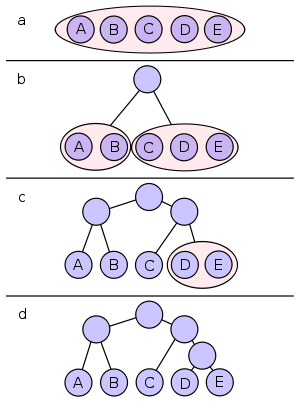
\includegraphics[width=0.5\linewidth]{images/shannon_fano_example.png}
	\caption[Shannon-Fano exaple tree]{Divide the list of symbols and assign code}
\end{figure}
\pagebreak
\begin{table}[h!]
  \begin{center}
    \pgfplotstabletypeset[
      	multicolumn names,
      	col sep=comma,
      	string type,
      	display columns/0/.style={column name=$Symbol$, column type={c}},
      	display columns/1/.style={column name=$Code$, column type={c}},
      	every head row/.style={before row={\toprule}, after row={\midrule}},
      	every row/.style={after row={\midrule}},
		every last row/.style={after row=\bottomrule},
    ]{tables/shannon-code.csv}
    \caption[Shannon-Fano exaple code]{The final code of symbols}
    \label{shannon-code}
  \end{center}
\end{table}
\subsubsection*{Pseudo-code}
You can find pseudo-code (Python style) for Shannon-Fano encoding and decoding in \textit{pseudo-code/shannon-fano.py}
\subsection{Lossless jpeg}
\paragraph*{Basic idea}
\paragraph*{Examples}
\paragraph*{Pseudo-code}
